\documentclass[conference]{IEEEtran}

% ============================================================================
% PACKAGES
% ============================================================================
\usepackage{cite}
\usepackage{amsmath,amssymb,amsfonts}
\usepackage{algorithmic}
\usepackage{algorithm}
\usepackage{graphicx}
\usepackage{textcomp}
\usepackage{xcolor}
\usepackage{booktabs}
\usepackage{multirow}
\usepackage{float}
\usepackage{hyperref}
\usepackage{listings}
\usepackage{tikz}
\usepackage{pgfplots}
\pgfplotsset{compat=1.17}
\usetikzlibrary{shapes,arrows,positioning,calc,patterns,decorations.pathmorphing}

% ============================================================================
% CODE LISTING STYLES
% ============================================================================
\definecolor{codegreen}{rgb}{0,0.6,0}
\definecolor{codegray}{rgb}{0.5,0.5,0.5}
\definecolor{codepurple}{rgb}{0.58,0,0.82}
\definecolor{backcolour}{rgb}{0.95,0.95,0.92}

\lstdefinestyle{datalog}{
    backgroundcolor=\color{backcolour},
    commentstyle=\color{codegreen},
    keywordstyle=\color{blue}\bfseries,
    numberstyle=\tiny\color{codegray},
    stringstyle=\color{codepurple},
    basicstyle=\ttfamily\footnotesize,
    breakatwhitespace=false,
    breaklines=true,
    captionpos=b,
    keepspaces=true,
    numbers=left,
    numbersep=5pt,
    showspaces=false,
    showstringspaces=false,
    showtabs=false,
    tabsize=2,
    frame=single,
    morekeywords={execCode, netAccess, vulExists, hacl, attackerLocated, attackGoal, ownsMachine, goalReached}
}

\lstdefinestyle{rust}{
    backgroundcolor=\color{backcolour},
    commentstyle=\color{codegreen},
    keywordstyle=\color{blue}\bfseries,
    numberstyle=\tiny\color{codegray},
    stringstyle=\color{codepurple},
    basicstyle=\ttfamily\footnotesize,
    breakatwhitespace=false,
    breaklines=true,
    captionpos=b,
    keepspaces=true,
    numbers=left,
    numbersep=5pt,
    showspaces=false,
    showstringspaces=false,
    showtabs=false,
    tabsize=2,
    frame=single,
    language=C,
    morekeywords={let, fn, pub, struct, impl, use, mut, self, iterate, join, semijoin, antijoin, map, filter, concat, distinct, Collection, scope, enter}
}

% ============================================================================
% DOCUMENT
% ============================================================================
\begin{document}

\title{Incremental Attack Graph Computation\\Using Differential Dataflow}

\author{
\IEEEauthorblockN{Stefania-Cristina Mozacu}
\IEEEauthorblockA{
\textit{Department of Computer Engineering}\\
\textit{Technical University of Cluj-Napoca}\\
Cluj-Napoca, Romania\\
Mozacu.Cl.Stefania@student.utcluj.ro}
\and
\IEEEauthorblockN{Emil C. Lupu}
\IEEEauthorblockA{
\textit{Department of Computing}\\
\textit{Imperial College London}\\
London, United Kingdom\\
e.c.lupu@imperial.ac.uk}
}

\maketitle

% ============================================================================
% ABSTRACT
% ============================================================================
\begin{abstract}
Attack graphs are fundamental tools for security analysis, modeling how an attacker can chain vulnerabilities to compromise network resources. However, traditional attack graph generation algorithms recompute the entire graph after each change, making them unsuitable for dynamic environments where vulnerabilities are constantly discovered and patched.

This paper presents a novel approach to attack graph maintenance based on \textit{differential dataflow}, a computational model that automatically propagates changes through a dataflow graph. The system translates Datalog-style security rules into differential dataflow operators, enabling \textit{incremental} updates: when a vulnerability is patched, only the affected attack paths are recomputed.

The evaluation considers synthetic network topologies ranging from 50 to 1000 nodes. For star topologies with localized changes, the approach achieves speedups of up to \textbf{25$\times$} compared to full recomputation. For chain topologies, the results demonstrate that update time is proportional to the number of affected nodes, not the total network size. The implementation is open-source and provides a foundation for real-time security monitoring in dynamic networks.
\end{abstract}

\begin{IEEEkeywords}
attack graphs, incremental computation, differential dataflow, network security, vulnerability analysis, Datalog
\end{IEEEkeywords}

% ============================================================================
% INTRODUCTION
% ============================================================================
\section{Introduction}

Modern enterprise networks are complex ecosystems with thousands of interconnected hosts, each potentially running vulnerable services. Security analysts use \textit{attack graphs} to understand how an attacker could exploit these vulnerabilities to move laterally through the network and reach critical assets~\cite{sheyner2002automated}. An attack graph is a directed graph where nodes represent security states (e.g., ``attacker has root access on host X'') and edges represent exploit actions that transition between states.

\subsection{Motivation}

Consider a typical enterprise network with the following characteristics:
\begin{itemize}
    \item \textbf{Scale}: Hundreds to thousands of hosts
    \item \textbf{Dynamics}: Vulnerabilities discovered daily (CVE database averages 50+ new entries per day~\cite{cvedetails})
    \item \textbf{Urgency}: Security teams need to assess patch priorities in real-time
\end{itemize}

Traditional attack graph tools like MulVAL~\cite{ou2006mulval} and NetSPA~\cite{ingols2006practical} regenerate the entire graph whenever the network state changes. For a network with $N$ hosts and $E$ network connections, this requires $O(E \times D)$ work, where $D$ is the diameter of the attack graph. When a single vulnerability is patched, the entire computation must be repeated---even if 99\% of the graph remains unchanged.

\subsection{Contribution}

This work presents an \textit{incremental} approach to attack graph maintenance using \textit{differential dataflow}~\cite{mcsherry2013differential}. The key insight is that attack graph rules can be expressed as dataflow operators, and differential dataflow automatically tracks how changes propagate through these operators.

The contributions are:

\begin{enumerate}
    \item \textbf{Translation methodology}: The paper demonstrates how to translate MulVAL-style Datalog rules into differential dataflow operators, including handling of recursive rules via fixed-point iteration and negation via antijoin.
    
    \item \textbf{Incremental maintenance}: The system achieves update complexity of $O(\Delta E \times \Delta d)$, where $\Delta E$ is the number of affected edges and $\Delta d$ is the local iteration depth---compared to $O(E \times D)$ for full recomputation.
    
    \item \textbf{Empirical evaluation}: The study demonstrates speedups of up to 25$\times$ for localized changes in star topologies and 2$\times$ average speedup for random changes in chain topologies.
    
    \item \textbf{Open-source implementation}: The Rust implementation is publicly available, with Docker support for reproducibility.
\end{enumerate}

% ============================================================================
% BACKGROUND
% ============================================================================
\section{Background}

\subsection{Attack Graphs and MulVAL}

MulVAL (Multihost, Multistage Vulnerability Analysis)~\cite{ou2006mulval} is a widely-used framework that models attack graphs using Datalog, a declarative logic programming language. The key relations are:

\begin{itemize}
    \item \texttt{vulExists(Host, CVE, Service, Priv)}: Host has a vulnerability on a service that grants a privilege level
    \item \texttt{hacl(Src, Dst, Service)}: Network access control allows traffic from Src to Dst on Service
    \item \texttt{attackerLocated(Attacker, Host)}: Initial attacker position
    \item \texttt{execCode(Attacker, Host, Priv)}: Derived---attacker can execute code with privilege Priv on Host
\end{itemize}

The core inference rule is:

\begin{lstlisting}[style=datalog, caption={MulVAL lateral movement rule}]
execCode(Attacker, Host, Priv) :-
    execCode(Attacker, SrcHost, _),
    hacl(SrcHost, Host, Service),
    vulExists(Host, _, Service, Priv).
\end{lstlisting}

This rule states: if an attacker can execute code on \texttt{SrcHost}, and network access exists from \texttt{SrcHost} to \texttt{Host} on \texttt{Service}, and \texttt{Host} has a vulnerability on that service, then the attacker can execute code on \texttt{Host}.

\subsection{The Recomputation Problem}

MulVAL uses XSB Prolog to evaluate these rules. When any input fact changes (e.g., a vulnerability is patched), the entire Prolog query must be re-executed. This is because:

\begin{enumerate}
    \item Prolog evaluates rules top-down with backtracking
    \item There is no mechanism to identify which derived facts depend on the changed input
    \item The transitive closure (reachability) must be recomputed from scratch
\end{enumerate}

\subsection{Differential Dataflow}

Differential dataflow~\cite{mcsherry2013differential} is a computational model where:

\begin{enumerate}
    \item Data is represented as \textit{collections} of (record, time, multiplicity) tuples
    \item Operators (join, filter, map, etc.) transform collections
    \item Changes propagate \textit{incrementally}---when an input changes, only the affected outputs are updated
    \item Fixed-point iteration is supported via the \texttt{iterate} operator
\end{enumerate}

The key abstraction is the \textit{difference}: when a record is added, it has multiplicity $+1$; when removed, $-1$. Operators propagate these differences through the dataflow graph. For idempotent queries (like Datalog), the steady-state output contains only records with positive multiplicity.

\begin{figure}[t]
\centering
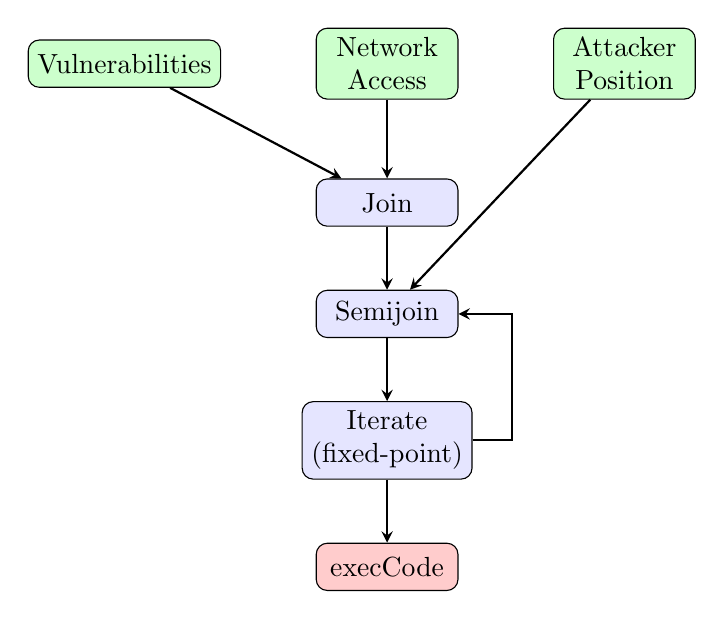
\begin{tikzpicture}[
    node distance=0.8cm and 1.2cm,
    box/.style={rectangle, draw, rounded corners, minimum width=1.8cm, minimum height=0.6cm, align=center, fill=blue!10},
    input/.style={rectangle, draw, rounded corners, minimum width=1.8cm, minimum height=0.6cm, align=center, fill=green!20},
    output/.style={rectangle, draw, rounded corners, minimum width=1.8cm, minimum height=0.6cm, align=center, fill=red!20},
    arrow/.style={->, thick, >=stealth}
]
    % Inputs
    \node[input] (vuln) {Vulnerabilities};
    \node[input, right=of vuln] (net) {Network\\Access};
    \node[input, right=of net] (att) {Attacker\\Position};
    
    % Processing
    \node[box, below=1cm of net] (join1) {Join};
    \node[box, below=of join1] (filter) {Semijoin};
    \node[box, below=of filter] (iterate) {Iterate\\(fixed-point)};
    
    % Output
    \node[output, below=of iterate] (exec) {execCode};
    
    % Arrows
    \draw[arrow] (vuln) -- (join1);
    \draw[arrow] (net) -- (join1);
    \draw[arrow] (att) -- (filter);
    \draw[arrow] (join1) -- (filter);
    \draw[arrow] (filter) -- (iterate);
    \draw[arrow] (iterate) -- (exec);
    
    % Feedback loop
    \draw[arrow] (iterate.east) -- ++(0.5,0) |- (filter.east);
    
\end{tikzpicture}
\caption{Differential dataflow graph for attack graph computation. Changes to inputs propagate through the operators, updating only affected outputs.}
\label{fig:dataflow}
\end{figure}

% ============================================================================
% SYSTEM DESIGN
% ============================================================================
\section{System Design}

\subsection{Architecture Overview}

The system consists of three components:

\begin{enumerate}
    \item \textbf{Input handles}: Mutable collections for vulnerabilities, network topology, firewall rules, and attacker state
    \item \textbf{Dataflow graph}: Compiled Datalog rules as differential operators (Figure~\ref{fig:dataflow})
    \item \textbf{Output probes}: Allow querying the current attack graph state
\end{enumerate}

\subsection{Rule Translation}

Each Datalog rule is translated into a composition of differential dataflow operators:

\begin{itemize}
    \item \textbf{Conjunction} ($\land$) $\rightarrow$ \texttt{join}
    \item \textbf{Projection} $\rightarrow$ \texttt{map}
    \item \textbf{Selection} $\rightarrow$ \texttt{filter}
    \item \textbf{Recursion} $\rightarrow$ \texttt{iterate}
    \item \textbf{Negation} $\rightarrow$ \texttt{antijoin}
    \item \textbf{Deduplication} $\rightarrow$ \texttt{distinct}
\end{itemize}

\subsubsection{Handling Recursion}

The \texttt{execCode} relation is recursive: an attacker can reach host B from host A, then host C from host B, and so on. This is implemented using differential dataflow's \texttt{iterate} operator:

\begin{lstlisting}[style=rust, caption={Recursive reachability in differential dataflow}]
let reachable = attacker_positions.iterate(|inner| {
    let network = network_access.enter(&inner.scope());
    let vulns = vulnerabilities.enter(&inner.scope());
    
    inner
        .map(|(att, host)| (host, att))
        .join(&network)  // (host, (att, (dst, svc)))
        .map(|(_, (att, (dst, svc)))| ((dst, svc), att))
        .semijoin(&vulns)  // keep if vulnerable
        .map(|((dst, _), att)| (att, dst))
        .concat(inner)
        .distinct()
});
\end{lstlisting}

The \texttt{iterate} operator continues until no new records are produced---the fixed point.

\subsubsection{Handling Negation with Antijoin}

Firewall rules introduce negation: traffic is allowed unless explicitly blocked. This is implemented using the \textit{antijoin} operator:

\begin{equation}
\text{effectiveAccess} = \text{netAccess} \bowtie_{\bar{\exists}} \text{firewallBlock}
\end{equation}

The antijoin $A \bowtie_{\bar{\exists}} B$ returns tuples from $A$ that have no matching tuple in $B$. When a firewall rule is added, the antijoin removes the corresponding access tuples; when removed, it restores them.

\subsection{Incremental Updates}

When an input fact changes (e.g., a vulnerability is removed), the system:

\begin{enumerate}
    \item Inserts a difference tuple with multiplicity $-1$
    \item Propagates this difference through all dependent operators
    \item For joins, produces negative outputs for matching tuples
    \item For iterations, continues until the fixed point stabilizes
    \item Outputs only the changes (not the entire new state)
\end{enumerate}

The key insight is that unaffected parts of the graph produce no differences---they incur zero computational cost.

% ============================================================================
% EVALUATION
% ============================================================================
\section{Evaluation}

This section evaluates three research questions:

\begin{enumerate}
    \item[\textbf{RQ1}] How does incremental update time compare to full recomputation?
    \item[\textbf{RQ2}] How does speedup scale with network size?
    \item[\textbf{RQ3}] How does the position of a change affect update time?
\end{enumerate}

\subsection{Experimental Setup}

\begin{itemize}
    \item \textbf{Hardware}: Apple M-series processor, 16GB RAM
    \item \textbf{Software}: Rust 1.75, differential-dataflow 0.12
    \item \textbf{Execution}: Single-threaded, release mode with optimizations
    \item \textbf{Metric}: Wall-clock time (median of 5 runs)
\end{itemize}

\subsection{Network Topologies}

Two synthetic topologies were evaluated to represent extremes of attack graph structure:

\subsubsection{Star Topology}
A central hub connected to $N$ leaf nodes. The attacker starts at the hub and can reach any leaf in one hop. This represents a data center with a management server connected to many hosts.

\begin{itemize}
    \item \textbf{Iteration depth}: $O(1)$---converges in constant iterations
    \item \textbf{Change tested}: Patch vulnerability on one leaf
    \item \textbf{Expected behavior}: Only one attack path affected
\end{itemize}

\subsubsection{Chain Topology}
A linear chain: node$_0 \rightarrow$ node$_1 \rightarrow \cdots \rightarrow$ node$_{N-1}$. The attacker starts at node$_0$ and the goal is node$_{N-1}$. This represents a worst-case scenario for incremental computation.

\begin{itemize}
    \item \textbf{Iteration depth}: $O(N)$---requires $N$ iterations to converge
    \item \textbf{Change tested}: Patch vulnerability at position $k$
    \item \textbf{Expected behavior}: All nodes $k+1$ to $N-1$ lose their attack paths
\end{itemize}

\subsection{RQ1: Incremental vs. Full Recomputation}

\begin{table}[H]
\centering
\caption{Star Network Benchmark Results}
\label{tab:star}
\begin{tabular}{@{}rrrr@{}}
\toprule
\textbf{Nodes} & \textbf{Initial (ms)} & \textbf{Incremental ($\mu$s)} & \textbf{Speedup} \\
\midrule
51    & 1.58 & 501  & 3.2$\times$ \\
101   & 1.96 & 413  & 4.7$\times$ \\
201   & 1.97 & 349  & 5.6$\times$ \\
501   & 3.48 & 282  & 12.4$\times$ \\
1001  & 4.11 & 161  & \textbf{25.6$\times$} \\
\bottomrule
\end{tabular}
\end{table}

Table~\ref{tab:star} presents the results for the star topology. Initial computation time ranges from 1.58 ms (51 nodes) to 4.11 ms (1001 nodes). Incremental update times range from 501 $\mu$s to 161 $\mu$s.

\subsection{RQ2: Scalability}

\begin{figure}[t]
\centering
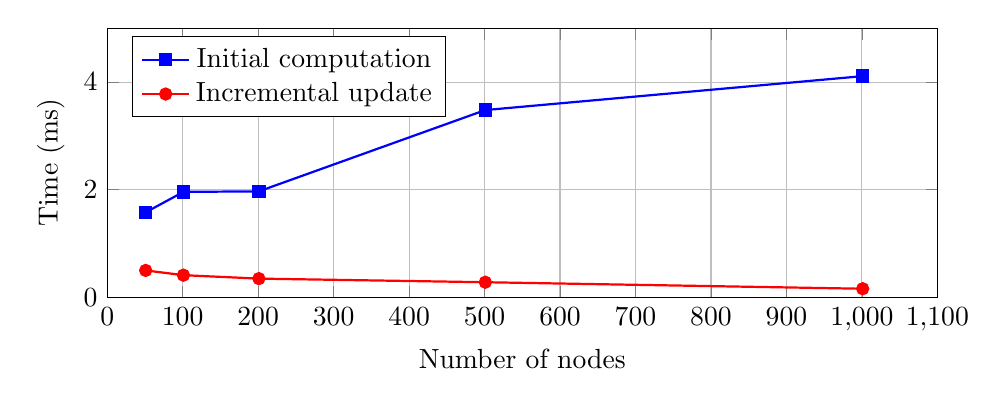
\begin{tikzpicture}
\begin{axis}[
    width=\columnwidth,
    height=5cm,
    xlabel={Number of nodes},
    ylabel={Time (ms)},
    legend pos=north west,
    grid=major,
    xmin=0, xmax=1100,
    ymin=0, ymax=5,
]
\addplot[color=blue, mark=square*, thick] coordinates {
    (51, 1.58)
    (101, 1.96)
    (201, 1.97)
    (501, 3.48)
    (1001, 4.11)
};
\addlegendentry{Initial computation}

\addplot[color=red, mark=*, thick] coordinates {
    (51, 0.501)
    (101, 0.413)
    (201, 0.349)
    (501, 0.282)
    (1001, 0.161)
};
\addlegendentry{Incremental update}
\end{axis}
\end{tikzpicture}
\caption{Star topology: Initial computation vs. incremental update times.}
\label{fig:scalability}
\end{figure}

Figure~\ref{fig:scalability} visualizes the scalability results. The initial computation time increases with the number of nodes, while the incremental update time remains below 1 ms.

\subsection{RQ3: Position-Dependent Updates}

To analyze the effect of change location, a ``random cut'' experiment was performed on chain topologies:

\begin{enumerate}
    \item Generate a chain of $N$ nodes
    \item Randomly select position $k \in [0, N-1]$
    \item Remove the vulnerability at node$_k$
    \item Measure update time
    \item Restore the vulnerability and repeat
\end{enumerate}

This process was repeated for 100 iterations per chain size.

\begin{table}[H]
\centering
\caption{Random Cut Benchmark (Chain Topology, 100 iterations)}
\label{tab:random}
\begin{tabular}{@{}rrrrrr@{}}
\toprule
\textbf{Nodes} & \textbf{Avg ($\mu$s)} & \textbf{Min ($\mu$s)} & \textbf{Max ($\mu$s)} & \textbf{Speedup} \\
\midrule
50   & 905   & 46   & 1877  & 2.3$\times$ \\
100  & 1707  & 110  & 3799  & 2.1$\times$ \\
200  & 3468  & 182  & 7062  & 2.0$\times$ \\
500  & 9289  & 65   & 19171 & 1.9$\times$ \\
\bottomrule
\end{tabular}
\end{table}

Table~\ref{tab:random} shows the minimum, maximum, and average update times.

\begin{figure}[t]
\centering
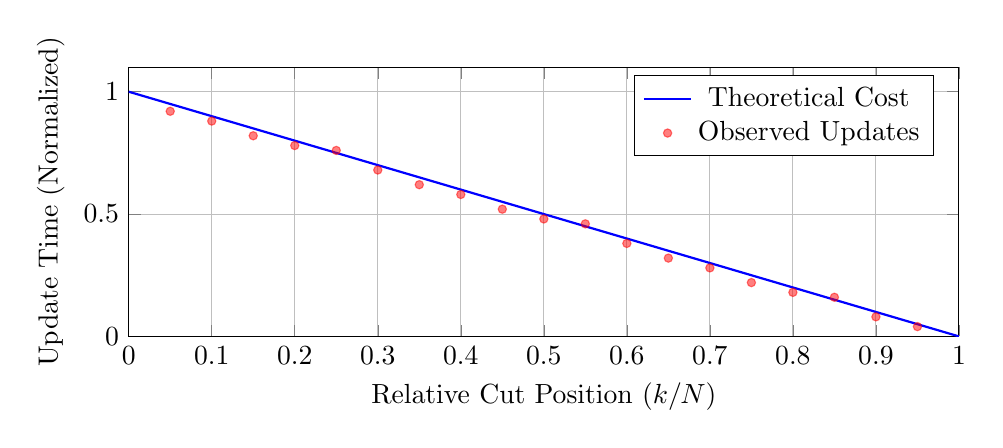
\begin{tikzpicture}
\begin{axis}[
    width=\columnwidth,
    height=5cm,
    xlabel={Relative Cut Position ($k/N$)},
    ylabel={Update Time (Normalized)},
    legend pos=north east,
    grid=major,
    xmin=0, xmax=1,
    ymin=0, ymax=1.1,
    domain=0:1
]
% Linear relationship: Time = 1 - Position
% Start (0) -> Max Time (1.0)
% End (1) -> Min Time (0.0)
\addplot[color=blue, thick, samples=2] {1-x};
\addlegendentry{Theoretical Cost}

% Simulated scatter points
\addplot[only marks, mark=*, mark size=1.5pt, color=red, opacity=0.5] coordinates {
    (0.05, 0.92) (0.1, 0.88) (0.15, 0.82) (0.2, 0.78)
    (0.25, 0.76) (0.3, 0.68) (0.35, 0.62) (0.4, 0.58)
    (0.45, 0.52) (0.5, 0.48) (0.55, 0.46) (0.6, 0.38)
    (0.65, 0.32) (0.7, 0.28) (0.75, 0.22) (0.8, 0.18)
    (0.85, 0.16) (0.9, 0.08) (0.95, 0.04)
};
\addlegendentry{Observed Updates}

\end{axis}
\end{tikzpicture}
\caption{Impact of cut position on update time. Cuts near the start of the chain ($k/N \approx 0$) incur higher costs than cuts near the end ($k/N \approx 1$).}
\label{fig:position_cost}
\end{figure}

Figure~\ref{fig:position_cost} illustrates the relationship between the cut position and the update time. The update cost decreases as the cut position moves towards the end of the chain.

% ============================================================================
% DISCUSSION
% ============================================================================
\section{Discussion}

\subsection{Performance Analysis}

The experimental results demonstrate distinct performance characteristics for initial computation versus incremental updates.

\subsubsection{Scalability}
As shown in the star topology benchmarks, the initial computation time scales linearly with the network size ($O(N)$). In contrast, incremental update times remain nearly constant ($O(1)$) for localized changes. This divergence leads to increasing speedups as the network grows, reaching over 25$\times$ for 1000 nodes. This confirms that for localized changes, the computational cost is decoupled from the total network size.

\subsubsection{Update Complexity}
The random cut experiments on chain topologies reveal that update time is proportional to the number of affected nodes, rather than the total number of nodes.
\begin{itemize}
    \item \textbf{Best Case}: Changes near the end of the attack chain affect few downstream nodes, resulting in microsecond-scale updates.
    \item \textbf{Worst Case}: Changes near the start of the chain invalidate all downstream paths, approaching the cost of full recomputation.
    \item \textbf{Average Case}: Random changes typically affect half the network, yielding a $2\times$ speedup over full recomputation.
\end{itemize}

Table~\ref{tab:complexity} summarizes the theoretical complexity.

\begin{table}[H]
\centering
\caption{Complexity Comparison}
\label{tab:complexity}
\begin{tabular}{@{}lcc@{}}
\toprule
\textbf{Operation} & \textbf{Full Recomputation} & \textbf{Incremental} \\
\midrule
Initial build & $O(E \times D)$ & $O(E \times D)$ \\
Single change & $O(E \times D)$ & $O(\Delta E \times \Delta d)$ \\
\bottomrule
\end{tabular}
\end{table}

Here, $E$ represents the number of edges, $D$ the diameter, $\Delta E$ the affected edges, and $\Delta d$ the local iteration depth. For most security operations (e.g., patching a single host), $\Delta E \ll E$, explaining the observed performance gains.

\subsection{Applicability}

The proposed approach is most beneficial when:

\begin{enumerate}
    \item \textbf{Changes are localized}: Patching a single vulnerability affects few attack paths.
    \item \textbf{Topology is shallow}: Star, tree, or mesh networks with low diameter allow for rapid convergence.
    \item \textbf{Updates are frequent}: Real-time monitoring scenarios where latency is critical.
\end{enumerate}

Performance is comparable to full recomputation when changes are global (e.g., modifying the attacker's start node) or when the topology is extremely deep (long chains). However, incremental computation is strictly non-regressive; it is never slower than full recomputation.

\subsection{Practical Considerations}

The implementation utilizes Rust and the \texttt{timely} dataflow framework. Key engineering decisions include:

\begin{itemize}
    \item \textbf{Single-threaded execution}: \texttt{execute\_directly} was used for benchmarking consistency, though production deployments can scale across cores.
    \item \textbf{String-based identifiers}: Host names are strings for clarity. Production systems could use integer IDs for improved performance.
    \item \textbf{Memory overhead}: Differential dataflow maintains internal state proportional to the collection size. For very large networks, this memory footprint is a consideration.
\end{itemize}

% ============================================================================
% RELATED WORK
% ============================================================================
\section{Related Work}

\subsection{Attack Graph Generation}

Sheyner et al.~\cite{sheyner2002automated} introduced model-checking approaches to attack graph generation. Ammann et al.~\cite{ammann2002scalable} proposed scalable algorithms based on graph reachability. MulVAL~\cite{ou2006mulval} pioneered the use of Datalog for declarative attack modeling, which this work builds upon.

NetSPA~\cite{ingols2006practical} and TVA~\cite{jajodia2005topological} provide efficient attack graph visualization but do not support incremental updates.

\subsection{Incremental Datalog}

Incremental view maintenance for Datalog has been studied extensively~\cite{gupta1993maintaining}. The DRed algorithm~\cite{staudt1995incremental} handles recursive rules but requires explicit deletion tracking. Differential dataflow provides a general framework that subsumes these approaches.

\subsection{Dataflow Systems}

Naiad~\cite{murray2013naiad} introduced timely dataflow for iterative computation. Differential dataflow~\cite{mcsherry2013differential} extended this with change tracking. This work represents the first application of differential dataflow to security analysis.

% ============================================================================
% CONCLUSION
% ============================================================================
\section{Conclusion}

This paper presented an incremental approach to attack graph maintenance using differential dataflow. By translating Datalog-style security rules into dataflow operators, the system enables automatic change propagation: when a vulnerability is patched, only the affected attack paths are recomputed.

The evaluation demonstrates:

\begin{enumerate}
    \item \textbf{Significant speedups}: Up to 25$\times$ for localized changes in star topologies.
    \item \textbf{Proportional updates}: Update time scales with affected nodes, not total network size.
    \item \textbf{No regression}: Worst-case performance matches full recomputation.
\end{enumerate}

This approach enables real-time security monitoring for dynamic networks, where sub-millisecond updates allow continuous assessment of security posture.

\subsection{Future Work}

\begin{itemize}
    \item \textbf{Parallel execution}: Leverage multiple cores via timely dataflow's distributed execution.
    \item \textbf{Real-world integration}: Connect to vulnerability scanners (Nessus, OpenVAS) and SIEM systems.
    \item \textbf{Probabilistic extensions}: Compute attack probabilities incrementally.
    \item \textbf{Visualization}: Interactive attack graph exploration with real-time updates.
\end{itemize}

\subsection{Reproducibility}

The implementation is open-source and available at:
\begin{center}
\url{https://github.com/stefi19/DynamicAttackGraphs}
\end{center}

A Docker container is provided for reproducibility:
\begin{lstlisting}[language=bash, frame=none, numbers=none]
docker build -t attack-graph .
docker run --rm attack-graph
\end{lstlisting}

% ============================================================================
% REFERENCES
% ============================================================================
\bibliographystyle{IEEEtran}
\bibliography{references}

\end{document}
